\chapter{Introduction}
\label{chp:introduction}

\nocite{*}

Powered by the decreasing process-node sizes, more efficient battery chemistry, and expanding wireless communication infrastructure, billions of Internet of Things (IoT) devices have entered our lives \cite{arif_2021, microsoft_2019}. However, the promise of ``smart dust'' seems to elude us still \cite{hester_2017}. In this vision, tiny internet-connected devices permeate our clothing, infrastructure, and more, enabling us to monitor everything \cite{marr_2018}.

One of the key aspects of wireless devices holding us back from this idea is the reliance on rechargeable, chemical batteries like those based on lithium. The lifespan of these batteries is severely limited by the number of charge cycles they can withstand before slowly reducing their total capacity. Moreover, even if they could maintain the same capacity throughout their entire lifespan, charging billions of sensor nodes is inconvenient, if not impossible, especially if they are embedded in concrete structures for maintenance monitoring purposes, for example.

The field of battery-free or batteryless computing aims to solve this by entirely ridding these devices of conventional batteries, opting to use capacitors as energy reserves instead \cite{freebie, hester_2017, satya_2019}. Capacitors provide numerous advantages compared to pouch or cylinder style lithium batteries, like tiny form factor, no leakage current, solid state architecture, and practically infinite lifetime, at least compared to other components within the device. 

Battery-free devices usually get their energy from harvesting. These sources could include solar (through photovoltaic cells) \cite{gameboy, colin_2018}, radio-frequency (through induction within the antennae) \cite{gollakota_2014, wisp_2005}, kinetic (e.g. by pressing buttons that capture kinetic energy) \cite{gameboy} and sometimes a combination of two or more methods. As one might imagine, these sources are sparse and can be unpredictable. 

\begin{figure}[]
    \centering
    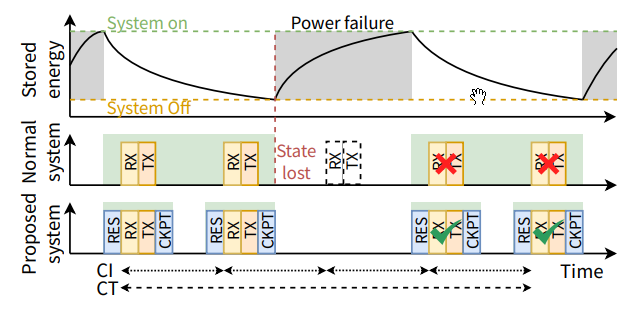
\includegraphics[width=0.8\textwidth,height=6cm,keepaspectratio=true]{images/intermittent_device_operation.png}
    \caption{
       Intermittently-powered device operation versus a conventionally-powered device operation (Figure taken from \cite{freebie}). When the conventional, non-protected system exhibits a power failure, all network state is lost, and the handshake procedure has to be fully restarted. An intermittently-powered device powers itself down in between network events in order to conserve energy as well as being able to fully recover from a power failure as if it was operating normally.
    }
    \label{fig:intermittent_operation}
\end{figure}

To conserve energy as much as possible, these devices often only power up parts of the system that are strictly necessary. This can take the form of the system only receiving power from its harvesting when being used (e.g., energy-harvesting buttons in smart light switches) or the system scheduling its own power-on events using low-power circuitry. This mode of operation is often called \textit{intermittent computing} and these devices \textit{intermittent} or \textit{intermittently-powered devices}. Figure \ref{fig:intermittent_operation} shows how these devices operate versus conventionally-powered devices.

Intermittently-powered operation makes wireless communication difficult. In the state-of-the-art solutions for intermittently-powered devices, Uni-directional communication has been achieved by advertising data when enough power is available. For example, bi-directional communication has been realized at a short range using RFID. With RFID technology, a reader ``interrogates'' a device that communicates back utilizing the principle of backscatter \cite{wisp_2005}. Although RFID is bi-directional, it requires a reader to energize the sensor devices at a short distance. As a result, medium-range, high throughput, intermittently-powered communication with active radios has not been possible until very recently. The system proposed by \cite{freebie}, called FreeBie, aims to solve this. It does so by using Bluetooth Low-energy and noting that, between transmission events, the System on Chip (SoC) could be powered down fully, only leaving on an ultra-low-power real-time clock (RTC) tasked with turning the SoC back on just in time for the next transmission. By doing so \cite{freebie} achieved the first ever battery-free devices capable of maintaining a wireless connection of a widely accepted standard. Even though BLE, as the name would suggest, has been developed for low-energy peripherals, its use within an intermittently-powered device has exposed some inefficiencies previously considered acceptable.

The work within this thesis will be based on the FreeBie system. By modifying the BLE stack source code, we aim to mitigate the inefficiencies of FreeBie. What these inefficiencies are will be discussed in the next section.

\section*{Problem Statement}
\label{sec:introduction_problem_statement}

To provide context, we would like to reiterate that intermittent devices receive power by harvesting ambient energy. Although the variability and unreliability of power is the root issue with energy harvesting systems, this can not be solved. However, it does provide context as to why the following issues do not exists with conventionally-powered BLE devices.

The first problem arises when the connection is formed. When the \textit{central}, for example, an Android phone, initiates a connection with a \textit{peripheral}, in this case FreeBie, it gets to decide the initial connection settings. These connection settings define the baseline connection speed and, as a result, the power consumption of the peripheral. After the connection setup, the peripheral can request more suitable connection parameters. However, this means that during the connection setup, we have to contend with the default connection parameters of the central. In the case of a phone running the Android operating system (OS), these settings are high-throughput and high power consumption. 

These unfavorable connection parameters forced FreeBie's designers to use capacitor sizes within FreeBie that, after the connection setup is finished, go mostly unused \cite{freebie}. This means the device as a whole increased in size and cost. 

The connection setup itself also has room for improvement. In the naive approach used in common frameworks, like Packetcraft and Zephyr, the connection setup is long and repetitive. For even a simple application, the number of packets required to setup can easily exceed 70 packets \ref{fig:division_packets}. At Android's fast settings, this already takes a few seconds. Using slower settings, which are more favorable for these ultra-low power devices, the setup can take up to three minutes. With more complex applications, these numbers increase rapidly.

Considering the variability of the power harvesting methods that these devices employ, it is often advantageous to switch to a faster connection configuration when plenty of energy is available or even crucial to switch to a slower connection configuration to protect against a power failure. Using the procedures available within the BLE specification, it takes a fixed six packets for the central to apply the connection settings after accepting them from the peripheral. This takes anywhere between tens of milliseconds to a minute, depending on the active connection parameters. 

Take as an example an intermittent device that takes its power from solar. If someone were to accidentally block the solar panel, then at the lowest connection settings, the device would not be able to throttle the connection fast enough to protect itself against a power failure. From all these remarks, we can gather at least three possible goals to improve BLE for use within intermittently-powered devices:
\begin{enumerate}
    \item \textbf{Goal 1}: Allow the Peripheral to dictate the initial connection parameters.
    \item \textbf{Goal 2}: Reduce the time required for the connection setup.
    \item \textbf{Goal 3}: Reduce the time required to apply new connection parameters.
\end{enumerate}
This thesis will address these the above three points with the general goal of improving the viability of BLE for intermittently-powered devices.

Chapter \ref*{chp:chapter_2} covers the necessary background information. Chapter \ref*{chp:chapter_3} will explain the architecture of the proposed solutions. Chapter \ref*{chp:chapter_4} validates and evaluates the efficacy of these solutions. Chapter \ref{chp:chapter_5} will draw a conclusion from the evaluation. Finally, Chapter \ref{chp:chapter_6} will discuss future work.
